% !TEX root = ../Projektdokumentation.tex
\section{Definition}
\label{sec:definition}


\subsection{Voraussetzungen} 
\label{sec:voraussetzungen}
Es gibt einige Voraussetzungen, die eine Wahl erfüllen muss, damit die \schulze auf diese Wahl angewendet werden kann.

\begin{enumerate}
\item Es muss mindestens zwei Kandidaten geben, die sich zu Wahl stellen, da sonst keine Rangfolge erstellt werden kann. Bei zwei Kandidaten ist die Lösung jedoch trivial, da dort der Gewinner der Kandidat ist, der am häufigsten, von den Wählern dem Gegner vorgezogen wurde.

\textbf{Mathematische Definition:}
Sei $A$ eine endliche nicht leere Menge an Kandidaten. Wobei die Anzahl der Kandidaten $C$ ist und gilt: 
\[
  C \in\ \mathbb{N}\  und \ 1 < C <\ \infty
\]

\item Jeder Wähler ordnet den Kandidaten eine Zahl zu und aus dieser Zahl wird eine Rangfolge erstellt. Je kleiner die Zahl ist desto höher ist die Platzierung. Hierbei ist die Größe der Zahl oder der Abstand uninteressant, da nur die Rangfolge betrachtet wird.

Des weiteren gilt:
\begin{enumerate}
\item \label{itm:Regel1} Es können mehrere Kandidaten die gleiche Platzierung haben, dass bedeutet, dass kein Unterscheidung der Kandidaten auf dieser Platzierung vorgenommen werden kann. 
\item Wenn ein Wähler keine Bewertung für einen Kandidaten abgibt, werden alle Kandidaten, die eine Bewertung haben, diesem Kandidaten vorgezogen. Werden mehrere Kandidaten nicht bewertet, werden sie wir im vorherigen Punkt gleich behandelt.
\end{enumerate}
\end{enumerate}

\subsection{Begriffsdefinition und Erläuterungen } 
\label{sec:begriffsdefinition}

Bevor die theoretische Definition aufgestellt werden kann, müssen einige Begriffe, Formeln und Notationen besprochen werden, um die Definition einfacher zu verstehen.


\subsubsection{Verbindung}
\label{verbindung}
Eine Verbindung in diesem Kontext bedeutet, dass zwei Kandidaten gegeneinander antreten und diese Duell ist eine Verbindung mit der folgender Notation

\[
(N[a,b],N[b,a])
\]
\textbf{Beispiel:}
Kandidat $a$ wird von fünf Wählern dem Kandidaten $b$ vorgezogen, und Kandidat $b$ wird von zwei Wählern Kandidat $a$ vorgezogen, würde wie folgt Notiert werden. 
\[
(5,2)
\]

In den Beispielen werden diese Duelle in einem Graphen dargestellt. Eine vollständigen Schreibweise, wie in Abbildung \ref{fig:verbindung1} skizziert, wird in Beispiel 3 benötigt.

\begin{figure}[!h]
\centering
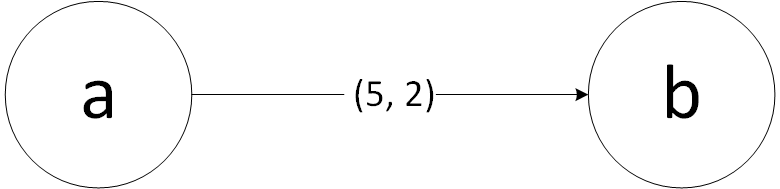
\includegraphics[scale=0.5]{Bilder/Definitionab.png}
\caption{Verbindung in Graphen}
\label{fig:verbindung1}
\end{figure}

In Fällen, in denen es nicht möglich ist Kandidaten gleich zu bewerten, wird auch die Kurzschreibweise wie in Abbildung \ref{fig:verbindung2} genutzt. Diese Darstellung wird auch in Beispiel 1 und in Beispiel 2 genutzt, da dort nicht wichtig ist, wie viele Gegenstimmen ein Siegreicher Kandidat bekommen hat.

\begin{figure}[!h]
\centering
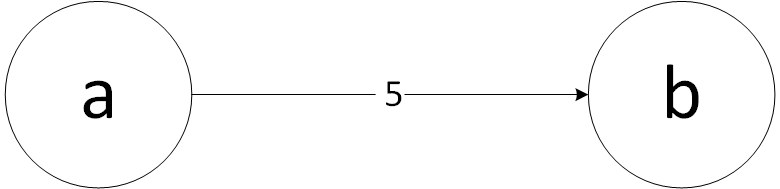
\includegraphics[scale=0.5]{Bilder/DefinitionShortab.png}
\caption{Verbindung in Graphen, Kurzschreibweise}
\label{fig:verbindung2}
\end{figure}

\newpage
\subsubsection{Weg}
\label{weg}
Ein Weg beschreibt Verbindungen zweier Kandidaten. Diese Kandidaten können direkt Verbunden werden oder auch über andere Kandidaten laufen. Dies wird wie folgt notiert.
\[
c(1),...,c(2)
\]

\textbf{Beispiel:} Kandidat $a$ schlägt Kandidat $b$ und Kandidat $b$ schlägt Kandidat $c$, dann schlägt Kandidat $a$ auch Kandidat $c$, da Kandidat $a$, Kandidat $b$ schlagen kann, auch wenn Kandidat $a$ nicht direkt Kandidat $c$ schlagen kann. Ein solcher Weg ist in rot in Abbildung \ref{fig:weg} aufgezeichnet. 

\begin{figure}[!h]
\centering
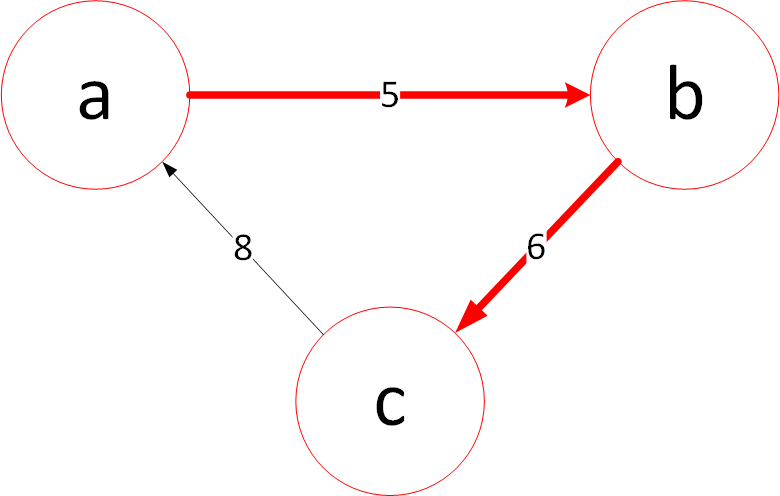
\includegraphics[scale=0.5]{Bilder/Weg.png}
\caption{Weg von $a$ über $b$ nach $c$}
\label{fig:weg}
\end{figure}

\subsubsection{Die Menge N}
\label{mengeN}
Die Menge $N$ kann man sich als Tabelle Vorstellen in der die Ergebnisse der Duelle der Kandidaten enthalten sind nach der ersten Auszählung. Die Menge $N$ ist die Grundlage der \schulze , auf diese Menge baut sich der Algorithmus auf. Ein Beispiel für diese Menge findet sich im Beispiel 1 in Tabelle \ref{Beispie1_N}.


\subsubsection{$\textsubscript{D}z$}
\label{dz}
Der Wert $_{D}z$ eines Weges ist der Wert, der die schwächste Verbindung repräsentiert. Das bedeutet, dass ein Weg untersucht wird und dort die schwächste direkt Verbindung zweier Kandidaten gesucht wird und dieser Wert wird als $_{D}z$ bezeichnet. Dieser Wert ist auch der ausschlaggebende Wert, der in  $P_{D}$ eingetragen wird. Wie eine schwache Verbindung definiert ist, ist abhängig von der gewählten Art der \schulze. Dies wird ausführlich im dritten Beispiel erläutert. Zum einfachen Verständnis kann anfangs ein einfacher Größenvergleich angenommen werden.
\newpage

\subsubsection{$P_{D}$}
\label{PD}
Diese Menge enthält die stärksten Wege zwischen den Kandidaten. Sprich die Wege, in denen die schwächste Verbindung ($_{D}z$) des Weges, stärker ist als alle anderen schwächsten Verbindungen von Wegen, die vom gleichen Kandidaten ausgehen und zum gleichen Kandidaten führen.

\subsubsection{Relation}
\label{relation}
\glqq Seien $A$ und $B$ Mengen. Eine Teilmenge $R$ enthalten in $A \times B$ heißt (zweistellige) Relation zwischen $A$ und $B$. Gilt $A = B$, so heißt $R$ Relation auf $A$.\grqq{} \citet{Lang2018}

Die \schulze nutzt die Relation $\mathcal{O}$, um dort die Ergebnisse der Duelle alle Kandidaten zu speichern, die sich aus der Menge $P_{D}$ ergeben. $P_{D}$ wird hier oft auch mit $P$ abgekürzt. Die  Relation $\mathcal{O}$ enthält dann nur die siegreichen Duelle. Ein siegreiches Duell $ab$ bedeutet, dass Kandidat $a$ gegen Kandidat $b$ gewonnen hat und ist in $\mathcal{O}$ enthalten.

\newpage
\subsection{Theoretische Grundlagen} 
\label{sec:theoretische Grundlagen}

Die grundsätzliche Idee der \schulze ist es, ein condorcetes Verfahren, wie in Abschnitt \ref{sec:condorectKriterium} beschrieben, durchzuführen. Dieses Verfahren wird jedoch über eine neue Berechnungsstufe verfeinert, um in einer Situationen einen Sieger zu ermitteln, in der die einfache \condorcetMethode keine Lösung liefert.

In diesem Abschnitt werden die Theoretischen Grundlagen erläutert und in den Abschnitten \ref{sec:beispiel1},  \ref{sec:beispiel2} und \ref{sec:beispiel3} an Beispielen erläutert.


\def\namedlabel#1#2{\begingroup
    #2%
    \def\@currentlabel{#2}%
    \phantomsection\label{#1}\endgroup
}

\begin{description}
\item[\namedlabel{itm:def231}{$(2.3.1)$}]  Ein Weg von Kandidat $x \in A$ zu Kandidat $y \in A$ ist eine folgen von Kandidaten $c(1),...,c(n) \in A$ mit den folgenden Eigenschaften:

\begin{center}
\begin{enumerate}
\item $x \equiv c(1)$
\item $y \equiv c(n)$
\item $2 \leq n \leq \infty$
\item Für alle $ i = 1,...,(n-1): c(i) \not\equiv c(i+1)$
\end{enumerate}
\end{center}


\item[\namedlabel{itm:def232}{$(2.3.2)$}]
Die Stärke eines Weges $c(1),...,c(n)$ ist $ min\textsubscript{D} \{(N[c(i),c(i+1)],N[c(i+1),c(i)])| i=1,...,n-1\} $.

In anderen Worten: Die Stärke eines Weges ist die Stärke der schwächsten Verbindung.

\item[\namedlabel{itm:def233}{$(2.3.3)$}]
Wenn ein Weg $c(1),..,c(n)$ die Stärke $z \in  \mathbb{N}_{0} \times \mathbb{N}_{0}$ hat, dann ist die kritische Verbindung dieses Weges, die Verbindung von  $(N[c(i),c(i+1)],N[c(i+1),c(i)]) \approx \textsubscript{D}z$.

\begin{align}
P_{D}[a,b] := max\textsubscript{D}\{ min\textsubscript{D} \{(N[c(i),c(i+1)],N[c(i+1),c(i)])| i=1,...,n-1\} \nonumber \\
     |c(1),...,c(n) \text{ ein Weg von Kandidat a zu Kandidat b}\} \nonumber
\end{align}

In andere Worten: $P_{D}[a,b] \in \mathbb{N}_{0} \times \mathbb{N}_{0}$ ist die Stärke des stärksten Weges von Kandidat $a \in A$ zu Kandidat $b \in A$.

\item[\namedlabel{itm:def234}{$(2.3.4)$}]Die zweistellige Relation $\mathcal{O}$ auf $A$ ist wie folgt definiert:
\[
ab \in \mathcal{O} : \Leftrightarrow P_{D}[a,b]>_{D}P_{D}[b,a]
\]
\item[\namedlabel{itm:def235}{$(2.3.5)$}] Daraus folgt, dass die Menge der Sieger sich wie folgt ergibt:

\[
\mathcal{S} := \{ a \in A | \forall b \in A \ \{a\}: ba \not\in \mathcal{O} \}
\]

\end{description}



